In this adaptation strategy, an initial solution is obtained on a baseline mesh with basic refinement zones that are usually used for a flow over an airfoil. We refer to this mesh as M0\_nz25, see Figure \ref{fig:M0_mesh}. 
Here nz25 refers to the number of spanwise extruded layers used in this mesh. 
For this mesh, the VMS-based error estimator is applied to phase-averaged data, and the maximum error value over all phases and the maximum in the spanwise direction (recall that we use an extruded mesh) for each element is selected to represent the error for that element throughout the surging cycle. 
The element-level error estimated on this mesh is shown in Figure \ref{fig:M0_err_plot}. 
We can see that higher errors are observed primarily in the region where the LEV traverses through the surging cycle, as well as in the wake of the airfoil. 
Higher errors are also observed close to the airfoil surface and in the boundary layer mesh region.

Based on estimated error, the mesh is refined by a factor of 2 in zones where high error values are found, including the boundary layer mesh in the streamwise direction. 
The spanwise resolution is also refined by a factor of 2 (i.e., the number of layers in the spanwise direction is doubled). 
This mesh, which is referred to as Mza1\_nz50 is shown in Figure \ref{fig:Mza1_mesh} and the estimated error is shown in Figure \ref{fig:Mza1_err_plot}. 
It is observed that the error has reduced by a factor of 4 in the Mza1\_nz50 mesh as compared to the M0 mesh.

%Zonal refinements are added to the Mza1 mesh in regions of high error, and the mesh is refined further by a factor of 2 in these zones, along with the boundary layer mesh in the streamwise direction, and the number of layers in the spanwise direction is doubled.  This mesh, which is referred to as Mza2, is shown in Figure \ref{fig:Mza2_mesh}. Again, we observe that the error has reduced by a factor of 4 in the Mz\_a2 mesh as compared to Mz\_a1 mesh.

The number of elements for each mesh is presented in Table \ref{table:mesh_zonal_summary}.

\begin{table}[H]
	\centering
	\caption{Summary of zonal refinement based meshes}
	\label{table:mesh_zonal_summary}
	\begin{tabular}{|l|c|c|c|c|c|}
		\hline
		Mesh case  & No. of elements\\
		\hline
		\hline
		M0\_nz25 & 774,525 \\
		\hline
		Mza1\_nz50 &  2,874,300 \\
		\hline
%		Mz\_a2 & 14,329,200 \\
%		\hline
	\end{tabular}
	
\end{table}

A detailed comparison of results based on these meshes is provided in Section \ref{sec:results_adapt}.

\begin{figure}[H]
\centering
\begin{subfigure}[b]{0.475\textwidth}
\centering
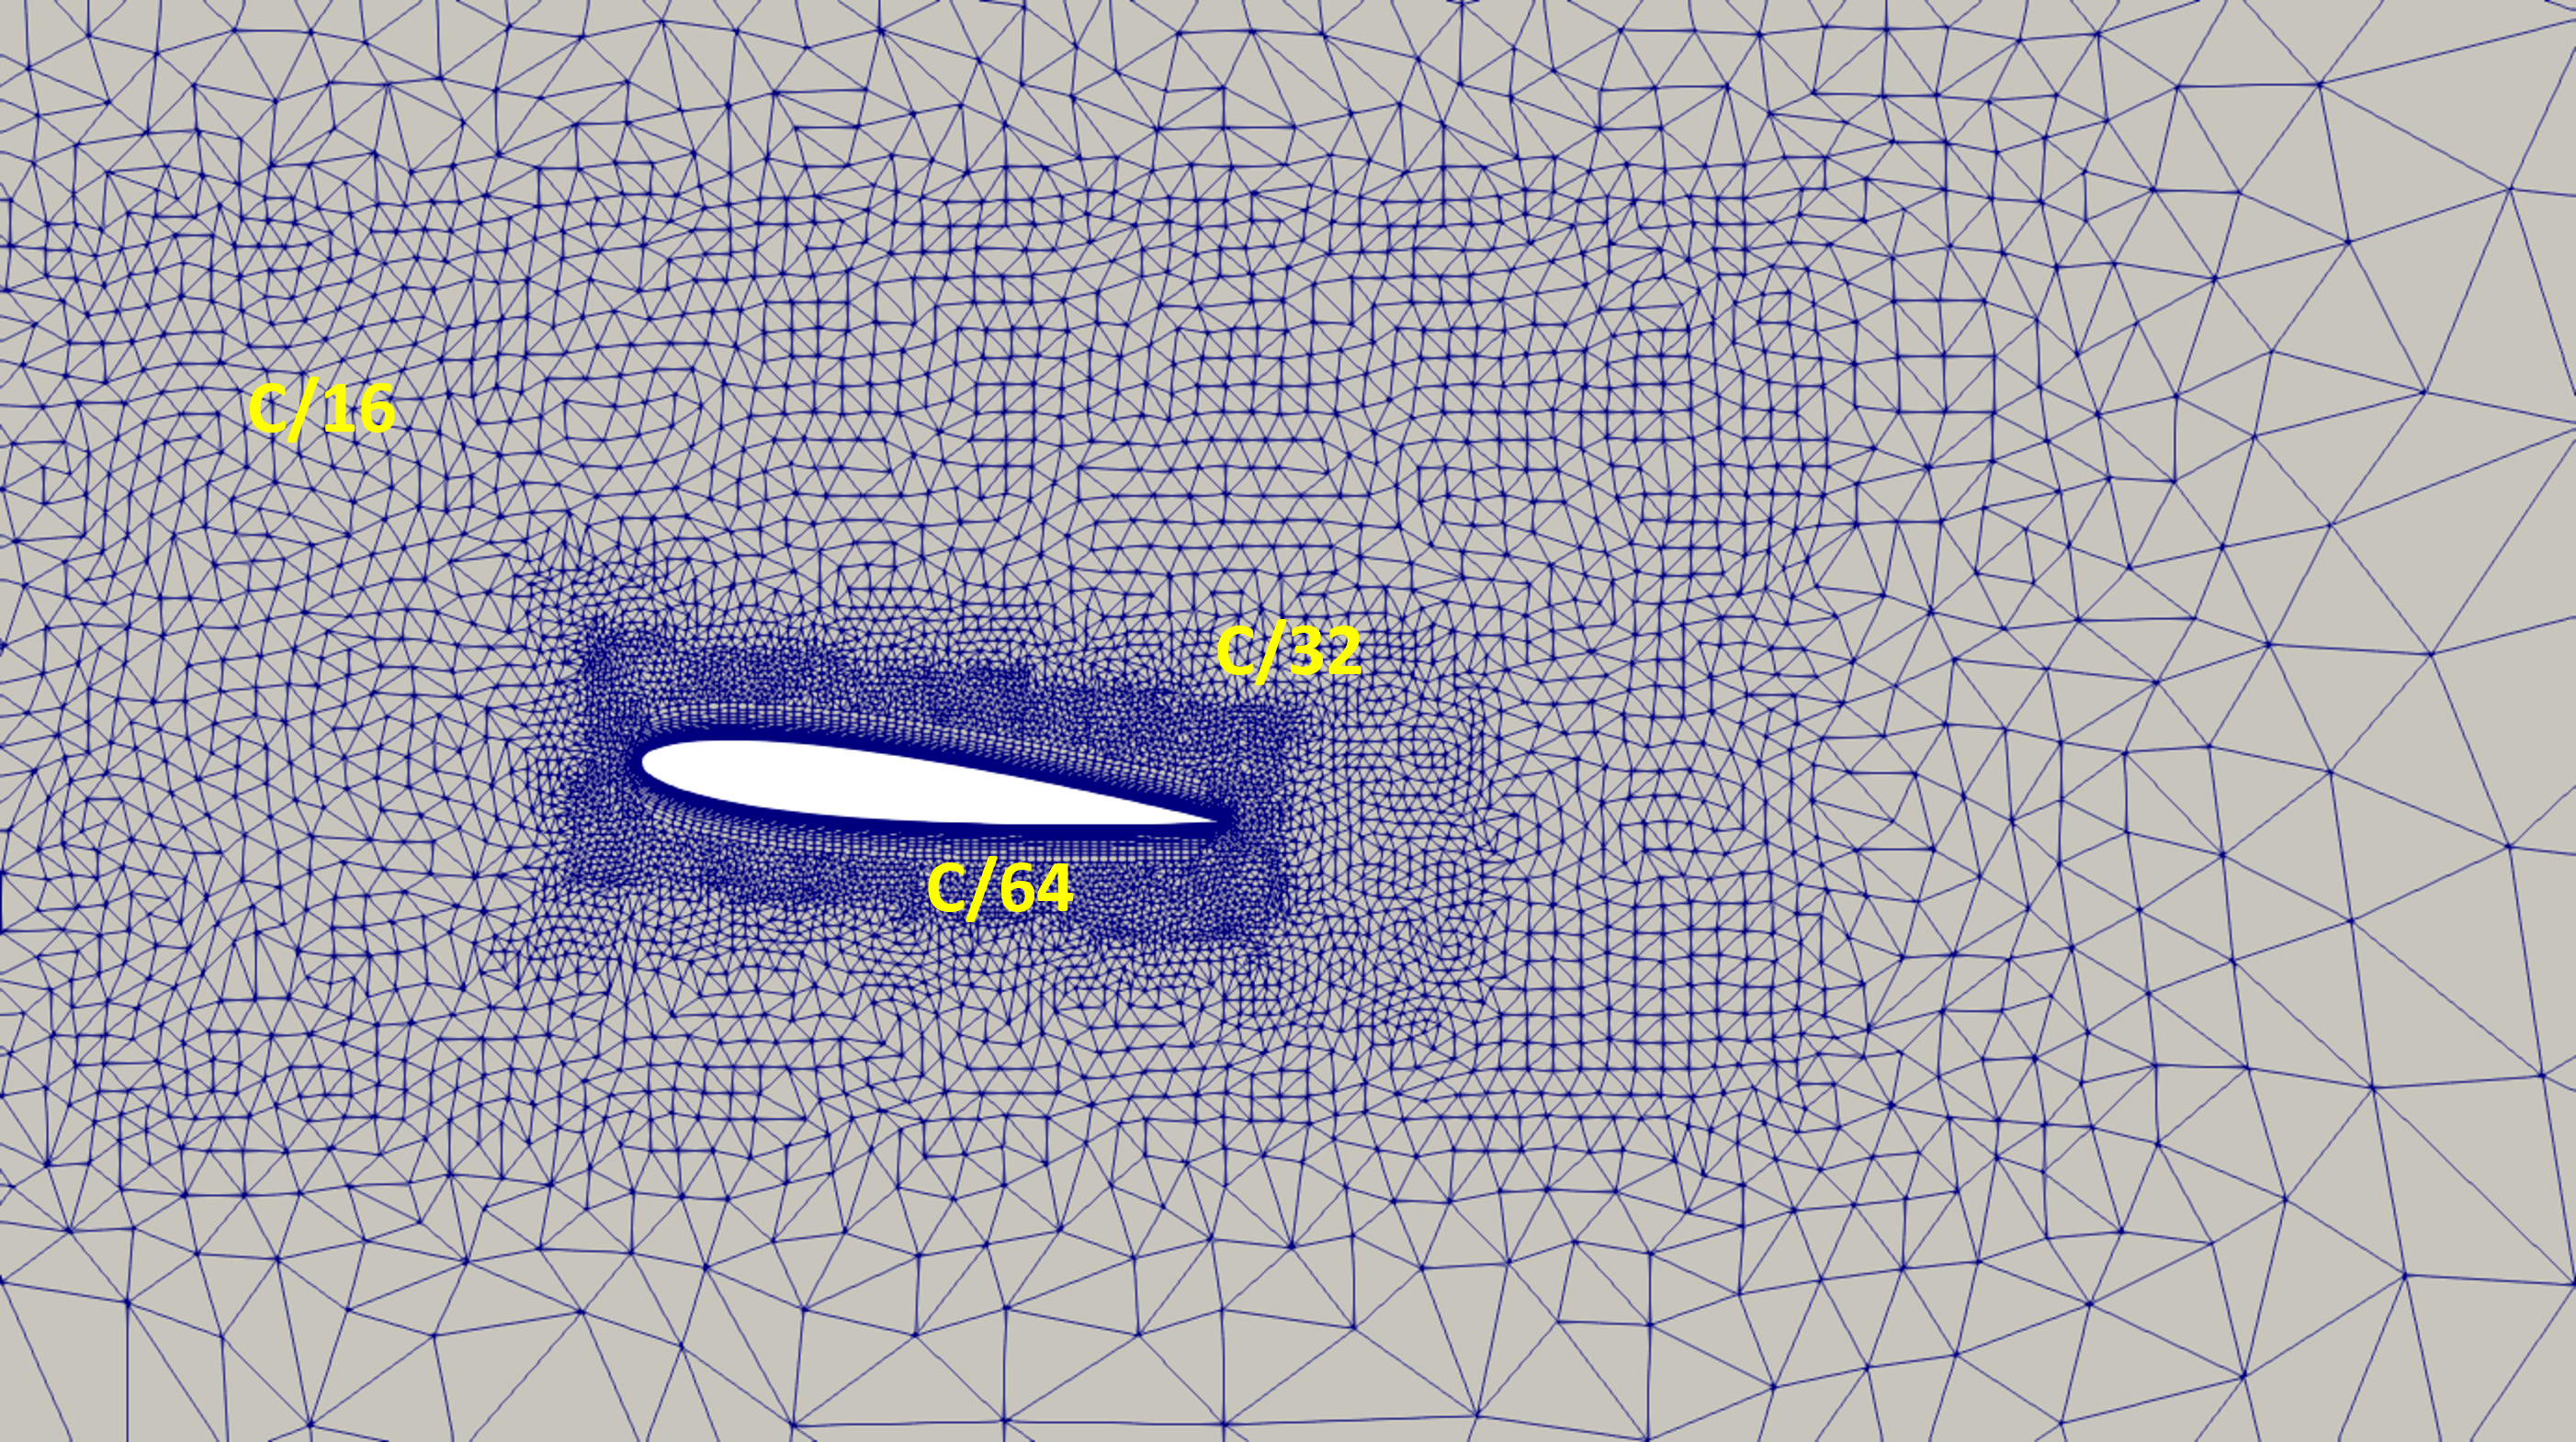
\includegraphics[width=1\textwidth]{figures/adapt_strat/M0_mesh.png}
\caption{M0\_nz25 mesh}
\label{fig:M0_mesh}
\end{subfigure}
\begin{subfigure}[b]{0.475\textwidth}
\centering
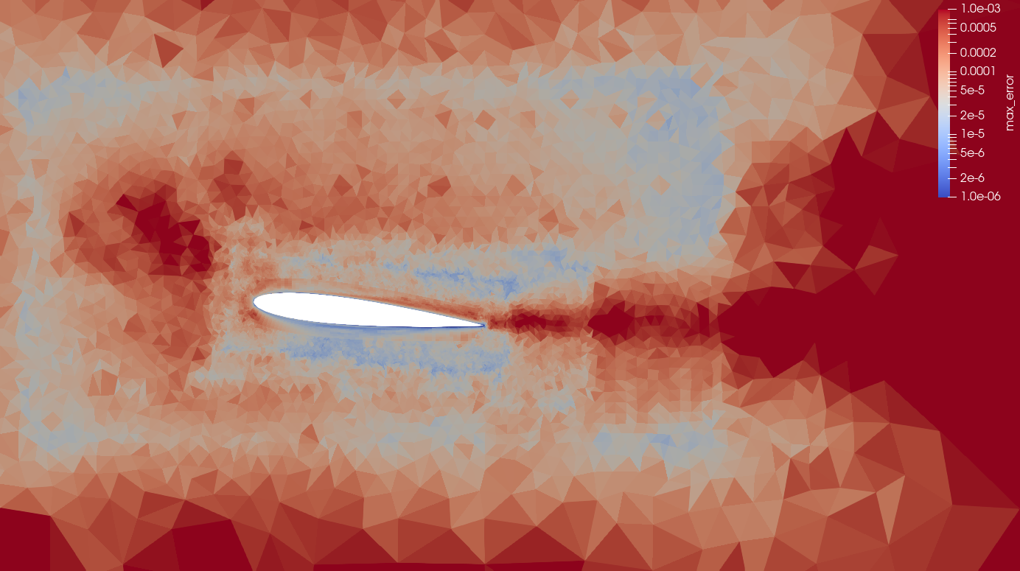
\includegraphics[width=1\textwidth]{figures/adapt_strat/M0_error_plot.png}
\caption{M0\_nz25 error field}
\label{fig:M0_err_plot}
\end{subfigure}
\begin{subfigure}[b]{0.475\textwidth}
\centering
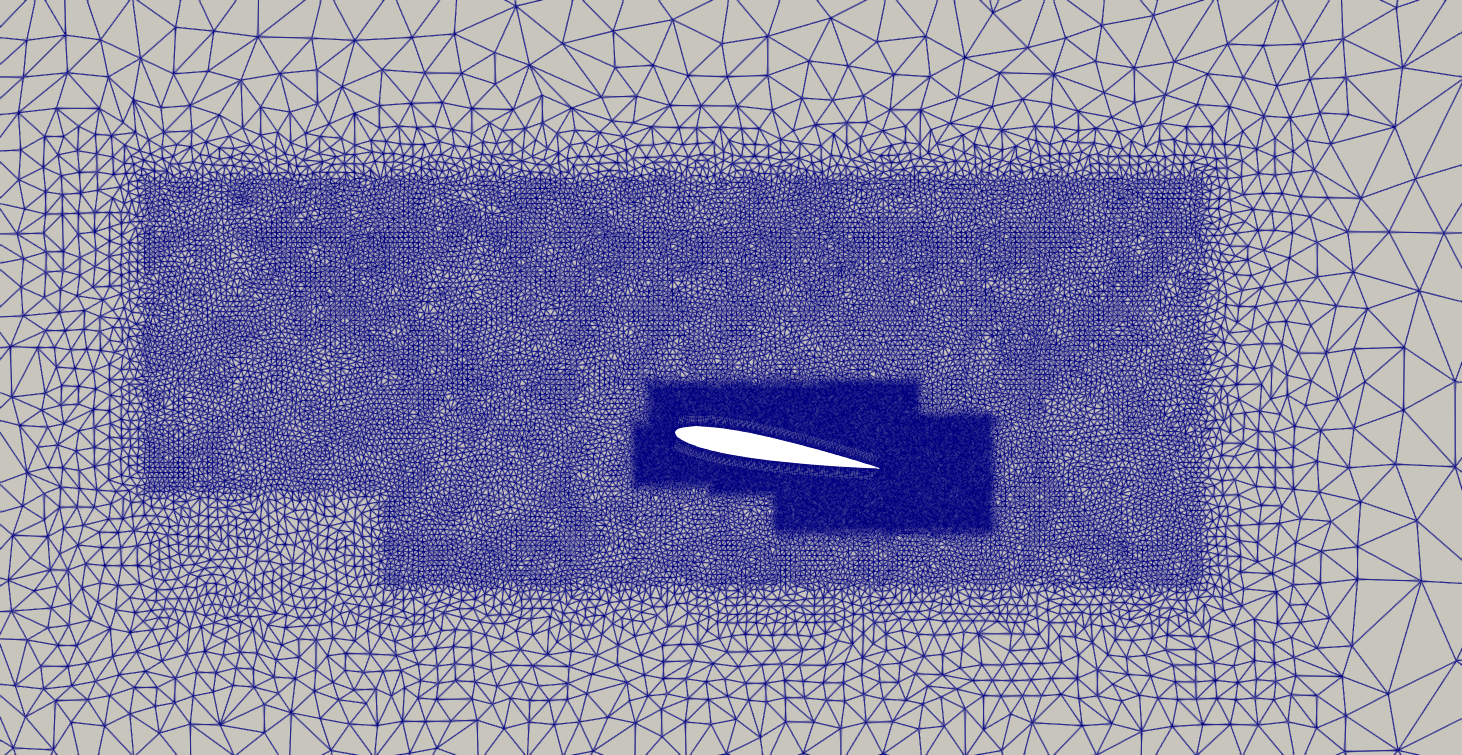
\includegraphics[width=1\textwidth]{figures/adapt_strat/Mza1_mesh.png}
\caption{Mza1\_nz50 mesh}
\label{fig:Mza1_mesh}
\end{subfigure}
\begin{subfigure}[b]{0.475\textwidth}
\centering
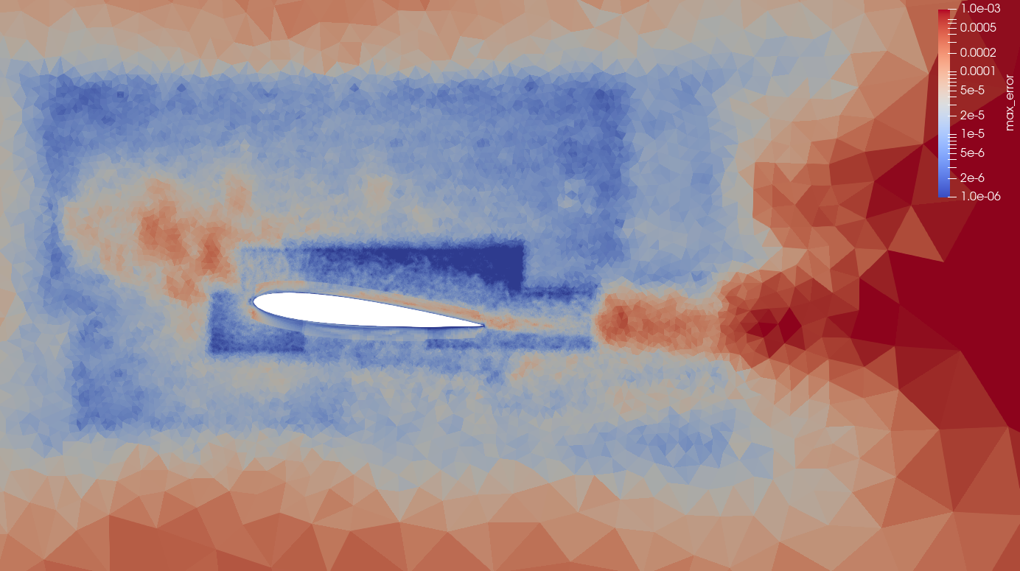
\includegraphics[width=1\textwidth]{figures/adapt_strat/Mza1_error_plot.png}
\caption{Mza1\_nz50 error field}
\label{fig:Mza1_err_plot}
\end{subfigure}
%\begin{subfigure}[b]{0.475\textwidth}
%\centering
%\includegraphics[width=1\textwidth]{figures/adapt_strat/Mza2_mesh.png}
%\caption{Mz\_a2 mesh}
%\label{fig:Mza2_mesh}
%\end{subfigure}
%\begin{subfigure}[b]{0.475\textwidth}
%\centering
%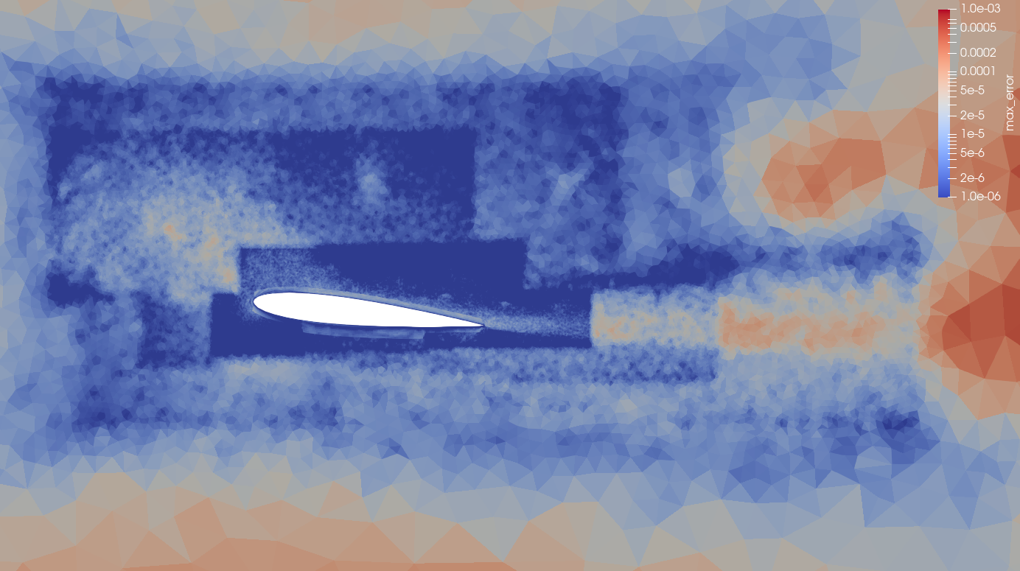
\includegraphics[width=1\textwidth]{figures/adapt_strat/Mza2_error_plot.png}
%\caption{Mz\_a2 error field}
%\label{fig:Mza2_err_plot}
%\end{subfigure}
\caption{Mesh and error-field for zonal based refinement strategy}
\end{figure}

